\documentclass{article}
\usepackage{tikz}
\usepackage{circuitikz}
\usetikzlibrary{shapes.gates.logic.US,shapes.gates.logic.IEC,positioning,calc,automata}
\begin{document}
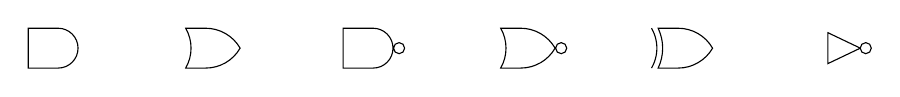
\begin{tikzpicture}
  \node[and gate US, draw, logic gate inputs=nn] (and1) at (0,0) {};
  \node[or gate US, draw, logic gate inputs=nn] (or1) at (2,0) {};
  \node[nand gate US, draw, logic gate inputs=nn] (nand1) at (4,0) {};
  \node[nor gate US, draw, logic gate inputs=nn] (nor1) at (6,0) {};
  \node[xor gate US, draw, logic gate inputs=nn] (xor1) at (8,0) {};
  \node[not gate US, draw] (not1) at (10,0) {};
\end{tikzpicture}
\end{document}
